%% Quran-Nazm paper, ACM format (acmart, sigconf). Full-paper version.
%% Build with pdflatex + bibtex (see README.md).
%% For submission switch the class options to [sigconf,review,anonymous] if the
%% call asks for double-blind review, and fill in the conference metadata.
\PassOptionsToPackage{table}{xcolor}
\documentclass[sigconf,nonacm]{acmart}

\usepackage{booktabs,multirow,tabularx}
\usepackage{subcaption}
\usepackage{tikz}
\usetikzlibrary{positioning,arrows.meta,decorations.pathreplacing}

\definecolor{nazm}{HTML}{2F6B55}
\definecolor{madina}{HTML}{C2412D}
\newcommand{\x}{\ensuremath{\times}}
\newcommand{\paperversion}{v0.4.0}% bump on each revision

\settopmatter{printacmref=false}
\setcopyright{none}

\begin{document}

\title{Quran-Nazm: Reducing Layout Variance in Quran Typesetting}
\titlenote{Paper version \paperversion.}

\author{Tarek Eldeeb}
\email{tarek.eldeeb@gmail.com}
\affiliation{%
  \institution{Quran-Nazm project}
  \city{Giza}
  \country{Egypt}
}

\begin{abstract}
Printed Qurans are organised in reading units (the juz, the hizb and its quarter, the rub') whose lengths differ widely: the longest rub' holds 2.19\x{} the text of the shortest. Any Mushaf that fixes how many pages a unit occupies must absorb this variance somewhere. The Madina Mushaf, written by Uthman Taha and composed by hand, fixes each juz to twenty pages and absorbs the rest line by line. Measuring all 8{,}790 full lines of its current (1441\,H) edition against a uniform DigitalKhatt reproduction of the hand, we find that a line holds 4 to 15 words, that its natural length ranges from 62\% to 136\% of the line width, and that one line in three is more than 10\% off; on the printed page, pen width varies by 13\% between lines and follows the crowding. We present \emph{Quran-Nazm}, an automatic typesetter that keeps the print's unit, twenty pages per juz, and absorbs the variance by rule instead of by hand: each juz is set as one natural line, cut into equal pages at ayah ends and equal lines at word boundaries by dynamic programming over shaped text widths, then justified with DigitalKhatt's letter elongation under a 19\% compression limit, with no surah title below line~11. Measured the same way on juz 1--29, the spread of line stretch falls from 0.104 in the print to 0.081 ($-22\%$), between the pages of a juz from 0.066 to 0.047 ($-28\%$) and within a page from 0.062 to 0.039 ($-37\%$). A stricter variant that fixes every hizb to ten pages, which we built first, evens lines within a page as well but leaves pages \emph{less} even than the print (0.086). Ablations and an exact solver checked against an integer programme show that the joint choice of page breaks is what keeps the pages even.
\end{abstract}

\ccsdesc[500]{Applied computing~Document preparation}
\ccsdesc[300]{Applied computing~Arts and humanities}

\keywords{Arabic typography, Quran, Madina Mushaf, line breaking, pagination, justification, kashida, DigitalKhatt}

\begin{teaserfigure}
  \centering
  \begin{subfigure}[b]{0.3\textwidth}\centering
    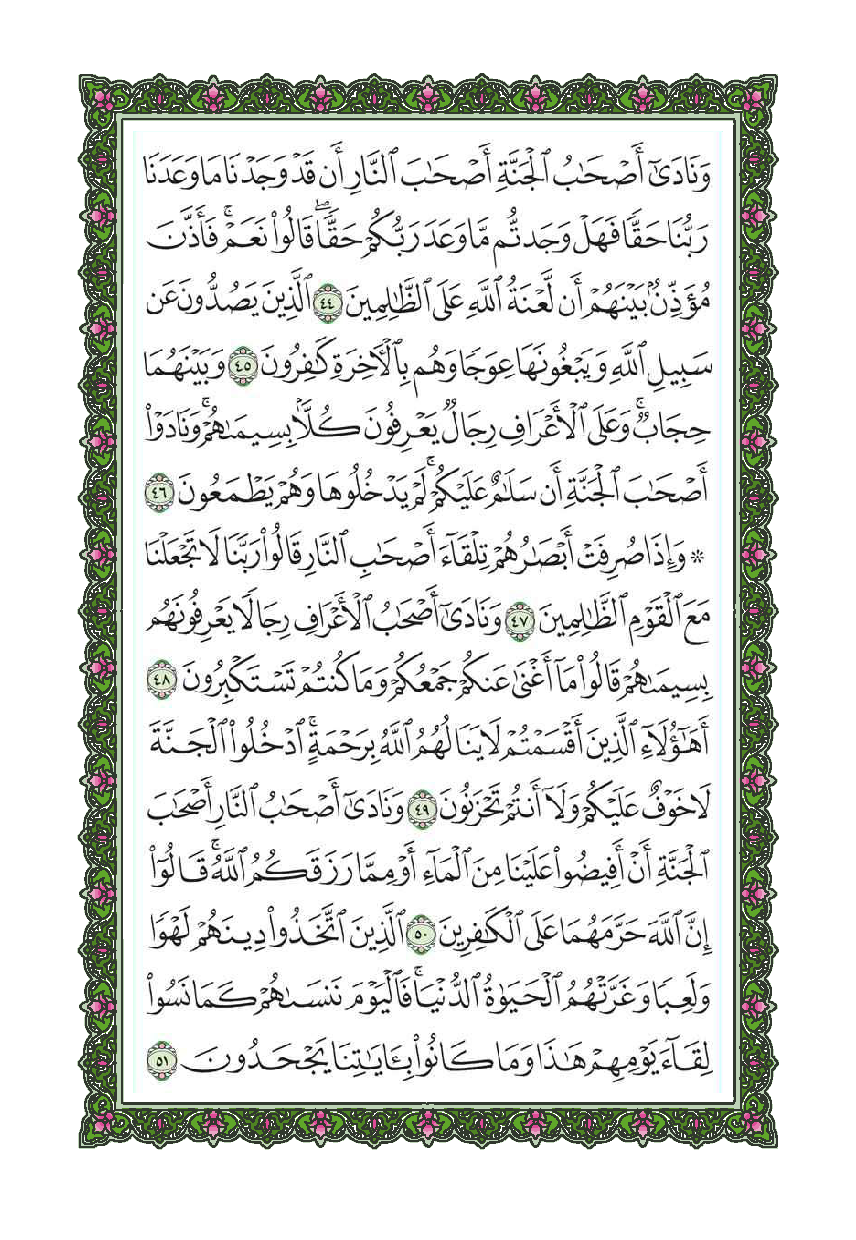
\includegraphics[width=\linewidth,trim=40 40 40 40,clip]{figures/madina-p156-framed.pdf}
    \caption{Madina 1441\,H print, page 156.}
  \end{subfigure}\hspace{8mm}%
  \begin{subfigure}[b]{0.3\textwidth}\centering
    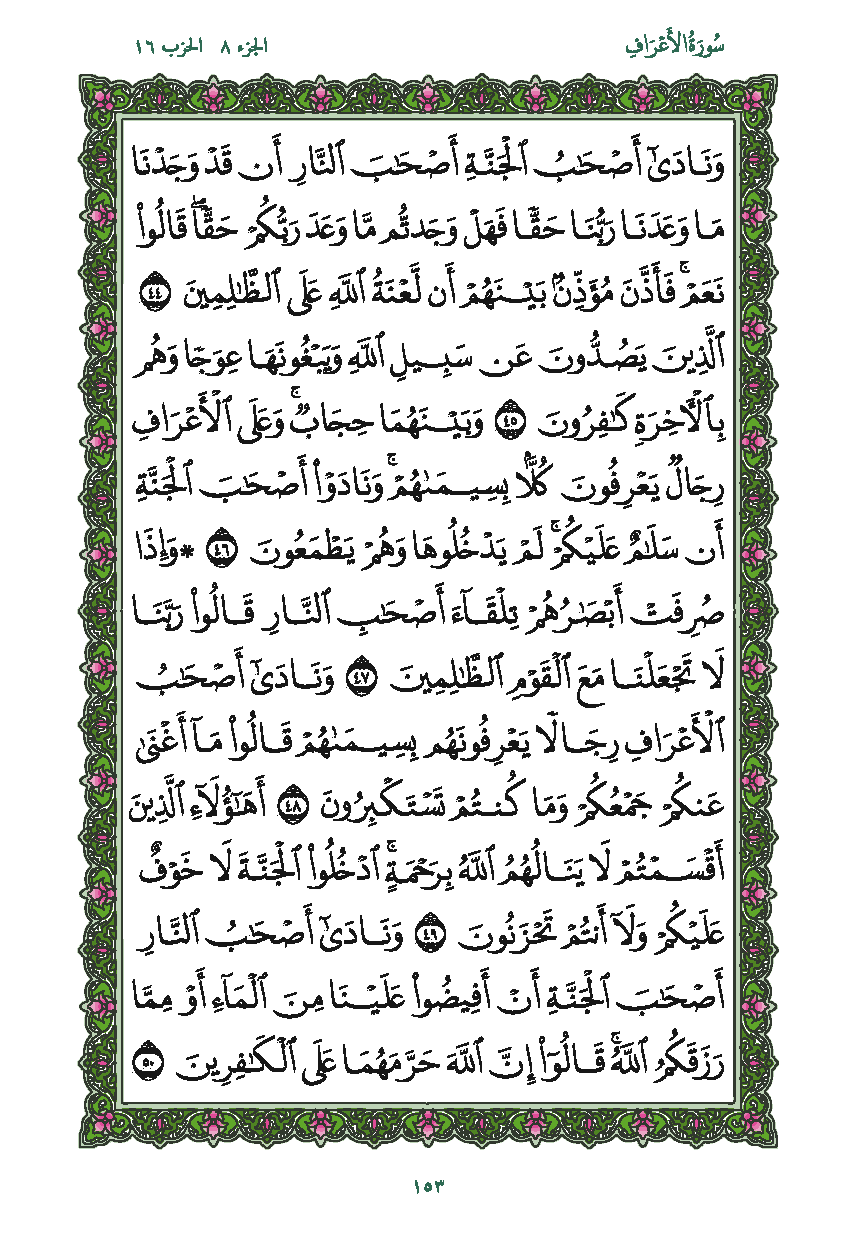
\includegraphics[width=\linewidth,trim=40 40 40 40,clip]{figures/nazm-p153.pdf}
    \caption{Quran-Nazm, page 153.}
  \end{subfigure}
  \Description{Two Quran pages side by side, both starting at the same ayah. Both pages sit in the same green Madina frame at the same size. The printed page has crowded lines at the top and spaced-out lines at the bottom; the Nazm page has evenly filled lines.}
  \caption{The same passage, from Al-A'raf 44, in the Madina print and in Quran-Nazm. In the print, line~11 carries 25\% more text than fits at natural size while the lowest lines are spaced out; in Nazm the lines of a page carry equal shares of text. For a fair comparison both text blocks are shown in the same Hafs frame at the same size (the print's text block is taken from the King Fahd Complex PDF~\cite{scan}), so only the setting differs.}
  \label{fig:teaser}
\end{teaserfigure}

\maketitle

\section{Introduction}
The Madina Mushaf has shaped how the Quran looks to readers for four decades. Its fifteen-line pages have become a shared map: readers memorise by page, teachers assign by page, and a juz, the thirtieth part of the Quran, begins at the top of a known page. The text was written by hand by Uthman Taha and the pages were then composed manually~\cite{kfgqpc}. The hand is the model that digital efforts try to reproduce; the composition is something else. Lines were filled by what fitted, stretched or compressed by eye, and in places the written words were scaled to close a line.

Behind these local decisions sits a global fact that every Mushaf faces: the traditional reading units are unequal. Their division is old: an early count of the Quran's letters, made to divide it into equal parts, is attributed to the time of al-Hajjaj ibn Yusuf al-Thaqafi (d.~95\,AH/714\,CE)~\cite{ibnabidawud,ibnkathir}. The Madina Mushaf does not follow al-Hajjaj's count. It takes the starts of its thirty juz, sixty hizbs and their quarters from \emph{Ghayth al-Naf`} by al-Safaqisi (d.~1118\,AH/1706\,CE), as the colophon of its Hafs edition states~\cite{kfgqpc1405}, and al-Safaqisi states his method. He does not compute the boundaries: where earlier authorities disagree on where a hizb begins, he follows ``only what is agreed upon or well known''. And he closes every quarter on a sound stop, naming its last word, the kind of stop it allows and whether it ends an ayah~\cite[p.~25]{safaqisi}; the first quarter of Al-Baqara, for instance, ends on ``a complete stop of the highest degree'', at an ayah end, ``by consensus''~\cite[p.~60]{safaqisi}. The units are thus drawn by meaning and tradition, not by length.

Drawn this way, the parts are far from equal in length (Section~\ref{sec:units}): a rub' (quarter of a hizb) may hold more than twice the text of another, and even the juz, the most even of the units, differ by 16\%. A Mushaf that wants a unit to begin at a fixed place must stretch some text and compress other text. The question is not whether to absorb this variance, but at which unit and by what means.

Digital Arabic typography has meanwhile reached the point where the Madina hand can be set by rule. DigitalKhatt~\cite{digitalkhatt,anane2021} models it as an OpenType font whose letters can elongate (kashida and alternate forms), and HarfBuzz~\cite{harfbuzz} shapes it on any platform. Our own renderer, quran-madina-html~\cite{qmh}, reproduces the existing Madina layouts line for line. This paper asks what a typesetter should do when it is free to choose the layout.

The question is not hypothetical. The Madina Mushaf is not frozen: its 1441\,H edition rebalanced lines and moved page breaks relative to the 1405\,H edition (Section~\ref{sec:problem}), and each revision is made by hand, in small steps. Quran-Nazm is an academic contribution to those revisions. It keeps what readers rely on, the twenty pages of each juz, the opening spread, the hand and the frame, and asks how far explicit rules can take the rest towards an optimal layout, and at what cost. Our contributions are:
\begin{enumerate}
  \item an analysis of the root variance, the unequal lengths of rub', hizb and juz, and of how fixing larger units reduces it (Section~\ref{sec:units});
  \item a quantitative account of how the Madina 1441\,H print absorbs the variance: line density, pen weight and ayah-marker placement (Section~\ref{sec:problem});
  \item Quran-Nazm, an open typesetter that fixes twenty pages per juz, like the print, and absorbs the variance by explicit rules on shaped text widths (Sections~\ref{sec:design} and~\ref{sec:impl});
  \item a three-way comparison of the print, a stricter ten-pages-per-hizb design and the juz design, which locates where each one leaves its variance (Section~\ref{sec:units-eval});
  \item an evaluation against the print, with ablations, an exact optimum and the cost of each rule (Section~\ref{sec:results}).
\end{enumerate}

\section{Related work}\label{sec:related}
\paragraph{Line breaking and pagination.} Knuth and Plass~\cite{knuth1981} cast line breaking as a global optimisation over all break points of a paragraph, solved by dynamic programming; \TeX{}~\cite{knuth1984} made it standard. Plass extended the idea to page breaks~\cite{plass1981}, and Mittelbach's framework for globally optimised pagination~\cite{mittelbach2016} and Woli\'nski's study of page breaking with column balancing~\cite{wolinski2019} bring it to complete documents. Hurst, Li and Marriott~\cite{hurst2009} survey automatic document formatting more broadly. Quran-Nazm applies the same principle at two levels, but with constraints specific to the Mushaf: a fixed number of pages per reading unit, page breaks only at ayah ends, surah titles kept away from the foot of a page, and a single line width for the whole book.

\paragraph{Arabic justification.} Latin justification stretches spaces; Arabic calligraphy stretches letters. Benatia, Elyaakoubi and Lazrek~\cite{benatia2006} survey the historical methods and propose an algorithm based on kashida; Haralambous~\cite{haralambous2006} describes infrastructure for high-quality Arabic typesetting; Anane~\cite{anane2021} justifies Arabic text in Lua\LaTeX{} with the variable DigitalKhatt font, whose letters elongate continuously. We use DigitalKhatt's elongation rules as ported in quran-madina-html~\cite{qmh}, and we examine its compression features in Section~\ref{sec:compress}.

\paragraph{Quran typesetting.} AlQalam~\cite{fahmy2006} extended ArabTeX for traditional Quranic text. The King Fahd Complex distributes its own fonts and vector page masters~\cite{kfgqpcdm}, and DigitalKhatt reproduces the Madina hand closely enough to re-set its layouts. These efforts reproduce existing layouts. To our knowledge, Quran-Nazm is the first to measure the layout variance of the Madina print, to compare page-count rules by where they leave that variance, and to replace manual composition with explicit, reproducible rules.

\section{The root variance: unequal reading units}\label{sec:units}
The Quran is divided into 30 juz, each of two hizbs, each of four rub'. These boundaries are part of the reading tradition; they mark where a daily portion or a recitation begins. They were not drawn to be equal in length, and they are not.

We measured every unit by its natural length: the sum of its words shaped once, without justification, in the QMH New Madina font (a patched DigitalKhatt font), plus normal spaces. Table~\ref{tab:unitlen} and Fig.~\ref{fig:units} show the result. The longest rub' (Al-Ma'ida 109 to Al-An'am 12) holds 2.19\x{} the text of the shortest (Al-Baqara 263--271); set at Madina size, rub' would need from 1.6 to 3.5 pages.

One way to remove this variance is to redefine the boundaries so that units hold equal text. That is a question for scholars of the reading tradition, not for typesetters, and it is out of scope here: a typesetter takes the boundaries as given.

The boundaries themselves show how they were drawn. Counting written letters, each juz starts on average within 2.3\% of a juz's length of its equal-letter position (at most 11\%), and juz lengths vary less (3.2\%) than they would if their quarters were independent (4.8\%): the juz were balanced as a whole. The quarters inside a juz were not. They sit on average 15\% of a quarter's length from the equal eighths of their juz, and up to 55\%, although cutting at the nearest ayah end could keep them within 2\%; 41 of the 240 open a surah. The quarters mark breaks in the text, a complete stop at an ayah end as al-Safaqisi requires, within juz that are close to equal.

What a typesetter can choose is the \emph{unit it holds fixed}. Variance falls as the unit grows, because the lengths of neighbouring rub' partly cancel. If rub' lengths were independent, the coefficient of variation of a unit of $n$ rub' would fall as $1/\sqrt{n}$; Table~\ref{tab:unitlen} shows that the measured values follow this trend, from 0.137 for the rub' to 0.077 for the hizb and 0.037 for the juz.

\begin{table}[t]
  \centering\small
  \caption{Natural length of the reading units at Madina type size. CV: coefficient of variation; predicted: rub' CV$/\sqrt{n}$.}
  \label{tab:unitlen}
  \begin{tabular}{@{}lrccccc@{}}
    \toprule
    Unit & $n$ & Count & Pages & Max/min & CV & Predicted \\
    \midrule
    Rub' & 1 & 240 & 1.6--3.5 & 2.19 & 0.137 & 0.137 \\
    Half hizb & 2 & 120 & 3.8--6.2 & 1.62 & 0.100 & 0.097 \\
    Hizb & 4 & 60 & 8.5--11.6 & 1.35 & 0.077 & 0.069 \\
    Juz & 8 & 30 & 18.6--21.5 & 1.16 & 0.037 & 0.049 \\
    \bottomrule
  \end{tabular}
\end{table}

\begin{figure}[t]
  \centering
  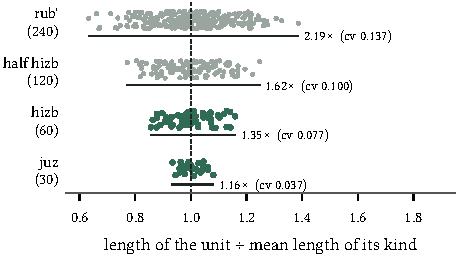
\includegraphics[width=\linewidth]{figures/fig_units.pdf}
  \Description{Four strips of dots, one per unit type, showing each unit's length divided by the mean length of its kind. The rub' strip spreads from about 0.6 to 1.4, the half hizb from 0.75 to 1.25, the hizb from 0.85 to 1.15 and the juz from 0.93 to 1.08.}
  \caption{The root variance. Each dot is one unit, its length relative to the mean of its kind; the spread narrows as units grow.}
  \label{fig:units}
\end{figure}

The Madina Mushaf standardises the largest unit. Each juz from 2 to 30 begins at or near the top of page $20k+2$: in the 1441\,H layout, 26 of these 29 juz start at the top of that page (18 on the first line, 8 under a surah header), and only 3 start within a page. Juz~1 occupies 21 pages and juz~30 occupies 23. Hizbs are only partly aligned: 38 of the 60 start at the top of a page (26 on the first line, 12 under a surah header), 5 more within its first three lines and 17 further down, and the distance from one hizb start to the next is 9, 10 or 11 pages (15, 29 and 15 times). Twenty pages per juz is the least demanding choice: the coefficient of variation of juz lengths is only 3.7\%.

A stricter choice is to fix every hizb to exactly ten pages, so that each hizb, not only each juz, begins on a known page. The first version of Quran-Nazm did this. Hizb lengths vary twice as much as juz lengths (Fig.~\ref{fig:hizb}), so more variance must be absorbed, and it must be absorbed within each hizb. Section~\ref{sec:units-eval} measures this trade on the finished layouts: the stricter unit costs more evenness than it buys, and Quran-Nazm therefore fixes the juz, as the print does, but absorbs the remaining variance by rule rather than by hand. The rest of the paper shows how the print absorbs its share, and how Nazm absorbs the same share by rule.

\begin{figure}[t]
  \centering
  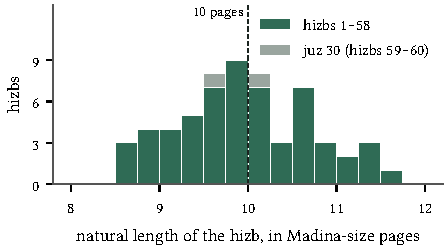
\includegraphics[width=\linewidth]{figures/fig_hizb.pdf}
  \Description{Histogram of the natural length of the 60 hizbs, between about 8.5 and 11.6 Madina pages, with a dashed line at 10 pages.}
  \caption{Natural length of the 60 hizbs at Madina type size. Fixing every hizb to ten pages would mean absorbing this spread inside each hizb.}
  \label{fig:hizb}
\end{figure}

\section{How the Madina print absorbs it}\label{sec:problem}
Within a juz of fixed length, the print still has to fill 300 lines of fixed width with text of uneven density. We measure how it did so, from three sources: the line breaks of the print, from the DigitalKhatt layout data used by quran-madina-html~\cite{qmh}; the printed pages themselves, from the King Fahd Complex PDF~\cite{scan}; and the Complex's QCF4 font, which traces every word of the print as a glyph~\cite{qcf4}.

\subsection{Line density}
Each full line of the print was shaped once, with no justification, and its natural length compared with the fixed line width. If the hand were set evenly, all lines would sit near 100\%. Fig.~\ref{fig:density} shows they do not: natural length runs from 62\% to 136\%; 15\% of lines are more than 10\% short and had to be stretched, and 18\% are more than 10\% long and had to be compressed. A full line holds 4 to 15 words and 21 to 52 letters.

Word count alone does not explain this. On page~72, lines 10, 11 and 12 each hold nine words, yet their natural lengths are $+11\%$, $-22\%$ and $+14\%$: word length matters as much as word count, which is why Nazm balances shaped widths and never counts words or letters. Page~156 (Figs.~\ref{fig:teaser}(a) and~\ref{fig:p156}) is the most uneven full page: most of its lines are overfull, up to $+25\%$ on line~11, while its last line is 15\% short, so the same hand appears compressed at the top of the page and spaced out at the bottom. Table~\ref{tab:madina} summarises the measurements of this section. The older 1405\,H edition, set from the same hand, is less balanced still: 38\% of its lines are more than 10\% off (27\% short, 11\% long) and the spread of stretch inside a page is 0.069, against 0.063 in 1441\,H. The revision rebalanced lines, but did not remove the variance.

\begin{figure}[t]
  \centering
  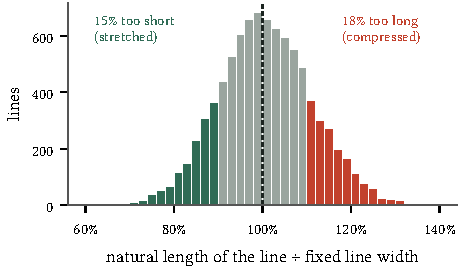
\includegraphics[width=\linewidth]{figures/fig_density.pdf}
  \Description{Histogram of the natural length of all full lines relative to the line width, from about 60 to 140 percent, with the tails below 90 and above 110 percent coloured.}
  \caption{Natural length of the 8{,}790 full lines of the 1441\,H print, relative to the line width. Coloured bars are lines more than 10\% off.}
  \label{fig:density}
\end{figure}

\begin{figure}[t]
  \centering
  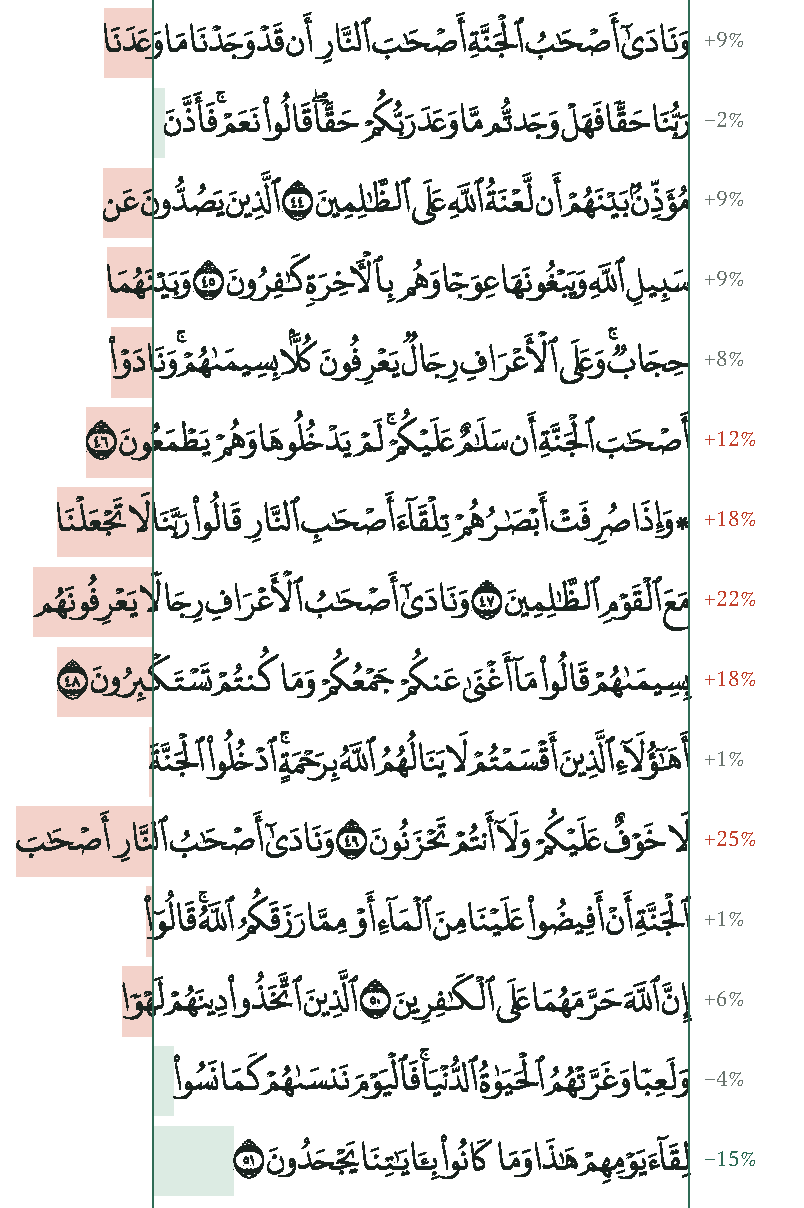
\includegraphics[width=0.92\linewidth]{figures/fig_p156_natural.pdf}
  \Description{Fifteen lines of Arabic text, each set at its natural length against two dashed vertical rules marking the printed line width; overlong lines are shaded red beyond the right rule and short lines leave a green gap, with a percentage per line.}
  \caption{Page 156 of the print, each line set once at its natural length in the DigitalKhatt reproduction of the hand. Dashed rules mark the printed line width; red shading is text that had to be compressed into it, green the gap that had to be filled.}
  \label{fig:p156}
\end{figure}

\begin{table}[t]
  \centering\small
  \caption{Layout variance measured on the Madina 1441\,H print. Pen figures: scan / QCF4 vector outlines.}
  \label{tab:madina}
  \begin{tabularx}{\linewidth}{@{}Xr@{}}
    \toprule
    Measure & Value \\
    \midrule
    Full-width lines measured & 8{,}790 \\
    Words / letters on a full line & 4--15 / 21--52 \\
    Natural length vs.\ line width & 62--136\% \\
    Lines off by more than 10\% & 33\% \\
    Pen width, light vs heavy line (5th--95th pct.) & +13\% / +12\% \\
    Pen width spread inside one page (median) & 9\% / 11\% \\
    Ink per letter, 5th--95th pct.\ (scan / vectors) & 1.36\x{} / 1.35\x \\
    Lines opening with an ayah marker & 573 (6.5\%) \\
    Surah titles below line 11 & 5 \\
    \midrule
    DK vs written width, recurring words ($r$) & 0.94 \\
    DK vs written width, per line ($r$) & 0.98 \\
    Spread inside a page: DK / written widths & 0.062 / 0.073 \\
    \bottomrule
  \end{tabularx}
\end{table}

\subsection{Is the font a fair yardstick?}\label{sec:yardstick}
Every stretch figure for the print rests on DigitalKhatt's natural width, a type designer's reconstruction of the hand rather than the hand itself. To test it against the calligrapher's own widths we used QCF4, the King Fahd Complex's font of the 1441\,H print, in which each word of each page is a glyph traced from the page~\cite{qcf4}. A glyph's ink width is the word's width as written on its line, with whatever elongation or scaling it received there. On the 8{,}515 full lines of juz 1--29 (74{,}911 words, matched one to one with the DigitalKhatt text), 68\% of the words belong to the 2{,}167 words that occur at least five times. For each of these, the median of its written widths over its occurrences estimates the calligrapher's natural width of that word.
\begin{itemize}
  \item \emph{Words.} The calligrapher's natural width follows DigitalKhatt's at $r=0.94$ on a log scale, with slope 0.96 and a residual of 0.12. That is about as much as one word varies between its own occurrences (median 0.10): the font disagrees with the hand by about as much as the hand varies.
  \item \emph{Lines.} Summed over the recurring words of a line, the calligrapher's natural width follows DigitalKhatt's at $r=0.98$ (residual 0.057), closer than the letter count does ($r=0.96$, residual 0.091).
  \item \emph{The print's stretch.} Measured with the calligrapher's widths (and DigitalKhatt's, rescaled, for the rarer words), the print's line stretch correlates with the DigitalKhatt measure at $r=0.83$. Its spread is 0.106 against 0.104; inside a page it is 0.073 against 0.062, and between pages 0.076 against 0.081.
\end{itemize}
So the unevenness of the print is not an artefact of the font: measured with the hand's own word widths it is as large overall, and larger inside a page. We keep the DigitalKhatt measure throughout, because it covers every word and is the same yardstick Nazm is set with; Nazm's own figures need no stand-in, since its lines are set in that font.

\subsection{Pen weight and texture}\label{sec:pen}
We measured pen weight from two sources, on the 7{,}305 full lines of the 487 pages of juz 1--29 made only of text. On the \emph{scan} (720\,\x\,1123\,px, about 100\,ppi) we split each page into its 15 line bands, masked the coloured ayah markers, upsampled each band four times and took the mean pen width as ink area divided by skeleton length. At this resolution a stroke is about two pixels wide, so we repeated every measurement on \emph{vector outlines}: the QCF4 glyphs of the same lines~\cite{qcf4}, rasterised at about 600\,ppi, where a stroke is about 13 pixels wide. The two agree line by line at $r=0.62$ for pen width and $r=0.87$ for ink per letter; a tracing may smooth the pen and a scan adds noise, so we report what both show (scan / vector):
\begin{itemize}
  \item a heavy line has a thicker stroke than a light one by 13\% / 12\% (5th to 95th percentile), and the heaviest line of a page is typically 9\% / 11\% heavier than its lightest;
  \item on page~102, line~5 is 16\% / 15\% heavier than line~4 directly above it (Fig.~\ref{fig:crops}(a));
  \item weight follows crowding (Fig.~\ref{fig:weight}): sparse lines (more than 10\% short), which were stretched, are written with 4\% / 7\% thicker strokes than crowded ones (more than 10\% long), and pen width correlates with crowding at $r=-0.36$ / $-0.61$. Ink per letter spans 1.36\x{} / 1.35\x{} (5th to 95th percentile) and correlates with crowding at $r=-0.61$ / $-0.68$. On page~192 a five-word line carries 65\% more ink per letter than a ten-word line of the same page (Fig.~\ref{fig:crops}(c)).
\end{itemize}
These line-level effects hold on both sources, and are stronger on the vectors. The likely mechanism is scaling of written words to fit: a line scaled up gains stroke weight as well as length. What does \emph{not} hold is a drift across the book. On the scan, weight falls over the first 500 pages ($r=-0.43$ with the page number) and rises by about 2\% in pages 540--580, where page~561 is 19\% heavier than page~563 (Figs.~\ref{fig:crops}(b) and~\ref{fig:drift}). On the vectors the fall is weaker ($r=-0.29$), there is no late rise, and page~561 is only 5\% heavier than page~563. We therefore attribute the late rise to the printing or scanning of those pages, not to the hand, and draw no conclusion from it.

\begin{figure*}[t]
  \centering
  \newcommand{\crop}[2]{\includegraphics[width=\linewidth]{figures/#1}\\[-1pt]{\scriptsize #2}\\[3pt]}
  \newcommand{\panel}[2]{\begin{minipage}[b]{0.485\textwidth}\centering #1{\footnotesize #2}\end{minipage}}
  \panel{\crop{madina-02-p-102-line-4.png}{p.\,102, line 4: pen 2.11\,px, 93\,px$^2$ ink per letter}%
         \crop{madina-03-p-102-line-5.png}{p.\,102, line 5: pen 2.45\,px (+16\%), 122\,px$^2$ ink per letter}}%
        {(a) Neighbouring lines written with different pens.}\hfill
  \panel{\crop{madina-04-p-561-line-9.png}{p.\,561, line 9: pen 2.85\,px, the heaviest page measured}%
         \crop{madina-05-p-563-line-9.png}{p.\,563, line 9: pen 2.14\,px, two pages later}}%
        {(b) The same line slot on nearby pages (a scan effect: 5\% on the vectors).}\\[8pt]
  \panel{\crop{madina-06-p-192-line-1-10-words.png}{p.\,192, line 1: 10 words, natural length 97\%, 89\,px$^2$ ink per letter}%
         \crop{madina-07-p-192-line-14-5-words.png}{p.\,192, line 14: 5 words, natural length 67\%, 147\,px$^2$ ink per letter (+65\%)}}%
        {(c) One page, two textures: a sparse line is stretched, enlarged and darkened.}\hfill
  \panel{\crop{madina-08-p-567-lines-2-3-ayah-marker-split.png}{p.\,567, lines 2--3: the last word of ayah 11 (left box) and its marker (right box)}}%
        {(d) An ayah's marker carried to the next line.}
  \Description{Seven crops of printed Quran lines in four panels showing different stroke weights between neighbouring lines, between nearby pages, between a crowded and a sparse line, and an ayah marker carried to the next line.}
  \caption{Anomalies in the Madina 1441\,H print: crops of the King Fahd Complex PDF~\cite{scan} at native resolution (about 100\,ppi). Measurements are those of Section~\ref{sec:problem}.}
  \label{fig:crops}
\end{figure*}

\begin{figure}[t]
  \centering
  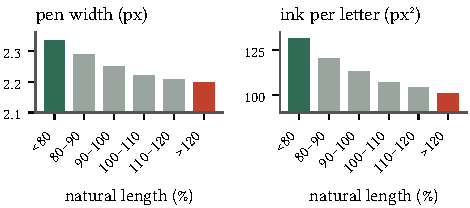
\includegraphics[width=\linewidth]{figures/fig_weight.pdf}
  \Description{Two bar charts: average pen width and average ink per letter both decrease as lines get more crowded.}
  \caption{Pen width and ink per letter on the scan, grouped by how crowded the line is (its natural length).}
  \label{fig:weight}
\end{figure}

\begin{figure}[t]
  \centering
  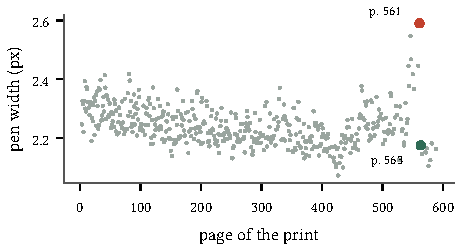
\includegraphics[width=\linewidth]{figures/fig_page_drift.pdf}
  \Description{Scatter plot of average pen width per page against page number. Values drift down from about 2.3 to 2.2 pixels over the first 500 pages, then rise, with page 561 the highest at about 2.6 and page 563 low at about 2.17.}
  \caption{Average pen width of each all-text page of the print, on the scan. The rise after page 540 does not appear on the vector outlines (Section~\ref{sec:pen}).}
  \label{fig:drift}
\end{figure}

\subsection{Ayah markers and surah titles}
In 573 lines (6.5\%) on 362 of the 604 pages, a line opens with the marker that closes the previous ayah, so the ayah ends at the far left of one line and its marker appears at the far right of the next (Fig.~\ref{fig:crops}(d)). All 440 such lines on the text-only pages were confirmed on the scan. This is an accepted convention of the print; we list it because a typesetter with more freedom can avoid it.

Five surah titles of the print sit on line 12 or 13 (pages 520, 587, 596, 599 and 602). In four of them the surah continues on the next page, so it opens with one or two lines at the foot of a page and breaks immediately. The print accepts this; Nazm forbids it (Section~\ref{sec:titles}).

\section{Design of Quran-Nazm}\label{sec:design}

\subsection{Which unit to fix}
Fixing a unit to a page count means choosing one line width for the whole book, wide enough for the densest unit; the other units must then stretch. Table~\ref{tab:fixed} shows the cost for each unit when nothing may be compressed. The rub' is impractical: type would fall to 56\% of the Madina size, and the shortest rub' would need 2.26\x{} stretch on average. The hizb is the smallest unit whose worst case stays within what DigitalKhatt elongates gracefully; the juz is by far the cheapest. Quran-Nazm fixes the juz to twenty pages, as the print does; the hizb alternative (ten pages per hizb) is kept as an option and compared in Section~\ref{sec:units-eval}. Juz~30, whose 37 short surahs each need a header, is the one exception, on 24 pages, which brings the book to 604 pages, the count of the print.

\begin{table}[t]
  \centering\small
  \caption{Fixed pages per unit, one common line width, no compression. Stretch is the average a unit's lines need.}
  \label{tab:fixed}
  \begin{tabular}{@{}lccc@{}}
    \toprule
    Unit $\to$ pages & Line width & Median & Worst \\
    & vs Madina & stretch & stretch \\
    \midrule
    Rub' $\to$ 2 & 1.78\x & 1.42\x & 2.26\x \\
    Half hizb $\to$ 4 & 1.61\x & 1.30\x & 1.68\x \\
    Hizb $\to$ 8 & 1.51\x & 1.22\x & 1.42\x \\
    Juz $\to$ 20 & 1.14\x & 1.15\x & 1.22\x \\
    \bottomrule
  \end{tabular}
\end{table}

\subsection{From one line to pages and lines}
Two constraints come from the tradition: a page ends at the end of an ayah, and no line starts with an ayah marker. Within them, the layout of a juz follows one idea (Fig.~\ref{fig:method}): \emph{set the whole juz as a single natural line, then cut it}.

\begin{figure}[t]
\centering
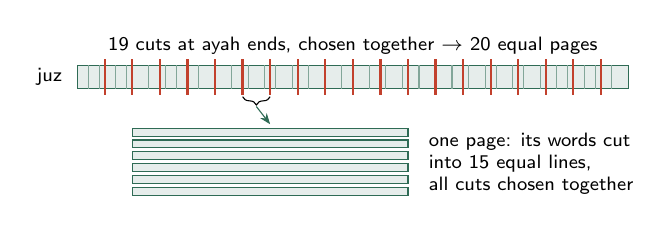
\begin{tikzpicture}[x=0.7cm,y=0.5cm,font=\sffamily\scriptsize]
  \node[anchor=east] at (-0.1,3.3) {juz};
  \fill[nazm!12] (0,3) rectangle (10,3.6);
  \draw[nazm] (0,3) rectangle (10,3.6);
  \foreach \t in {0.2,0.4,0.7,0.9,1.3,1.6,1.8,2.2,2.5,2.8,3.1,3.4,3.6,3.9,4.2,4.5,4.8,5.3,5.6,5.9,6.2,6.5,6.8,7.1,7.4,7.6,7.9,8.1,8.4,8.7,8.9,9.2,9.4,9.7} \draw[nazm!60] (\t,3) -- (\t,3.6);
  \foreach \c in {0.5,1,...,9.5} \draw[madina,thick] (\c,2.85) -- (\c,3.75);
  \node at (5.0,4.1) {19 cuts at ayah ends, chosen together $\rightarrow$ 20 equal pages};
  \draw[decorate,decoration={brace,amplitude=3pt,mirror}] (3.0,2.8) -- (3.5,2.8);
  \draw[-{Stealth[length=1.4mm]},nazm] (3.25,2.55) -- (3.5,2.1);
  \foreach \i in {0,...,5} {\fill[nazm!12] (1.0,1.8-0.3*\i) rectangle (6.0,2.0-0.3*\i); \draw[nazm] (1.0,1.8-0.3*\i) rectangle (6.0,2.0-0.3*\i);}
  \node[anchor=west,align=left] at (6.2,1.1) {one page: its words cut\\into 15 equal lines,\\all cuts chosen together};
\end{tikzpicture}
\Description{A long bar representing a juz set as one natural line, with thin ticks at ayah ends and nineteen red cuts dividing it into twenty equal pages; one page below is divided into equal lines.}
\caption{The layout idea: a juz is one natural line, cut into twenty equal pages at ayah ends, and each page into equal lines at word ends.}
\label{fig:method}
\end{figure}

Let the juz consist of ayahs $1..N$ with natural widths $a_k$ (shaped words plus spaces, each marker glued to its preceding word), and let a surah header count as $h_k\in\{0,1,2\}$ lines of width $q$, the juz's average text per line. With cumulative widths $V_k=\sum_{i\le k}(a_i+h_iq)$ and target $\bar V=V_N/20$, the page cuts $0=c_0<c_1<\dots<c_{20}=N$ at ayah ends minimise
\begin{equation}
  \sum_{p=1}^{20}\bigl(V_{c_p}-V_{c_{p-1}}-\bar V\bigr)^2+\sum_{p}\pi(c_p),
  \label{eq:pages}
\end{equation}
where $\pi$ penalises a cut inside a surah short enough for one page, subject to the title rule below. Each page holds $L=15-H$ text lines after its $H$ header lines; every surah on the page starts on a new line, and the page's lines are shared among its surah segments so that none is crowded. A segment of words $w_1..w_m$ is then cut into its $L'$ lines $\ell$ of natural width $w_\ell$ by minimising
\begin{equation}
  \sum_{\ell=1}^{L'}\bigl(w_\ell-\bar w\bigr)^2,\qquad \bar w=\tfrac{1}{L'}\textstyle\sum_\ell w_\ell,
  \label{eq:lines}
\end{equation}
over word boundaries. Both problems are solved exactly by dynamic programming, in the spirit of Knuth and Plass~\cite{knuth1981}, with a sum-of-squares cost. All widths are HarfBuzz advances in the DigitalKhatt font; the method never counts words or letters. Hizb boundaries play no part: they fall wherever the text puts them and only label the running heads.

\subsection{The opening spread}\label{sec:opening}
Every printed Mushaf opens with a decorated spread: Al-Fatiha on the right page and Al-Baqara 1--5 on the left, each in a small block whose lines narrow towards its top and bottom, inside a larger ornament. Nazm keeps this tradition. The two pages are labelled \emph{alif} and \emph{b\=a'}, and the page numbers start after them, so that page~1 is the first full page, Al-Baqara~6. The spread counts as two of juz~1's twenty pages: the rest of juz~1 takes 18 full pages, and the book has 602 numbered pages, 604 in all, like the print. On each opening page the line widths follow the shape of the print's (from 36\% to 83\% of the line width), scaled so the lines keep the book's median stretch of 1.07\x, and the line breaks are chosen by dynamic programming to fit that shape. The opening ornament of quran-assets is not yet traced, so Nazm draws a double outline that follows the lines. With twenty full pages, juz~1 would have been the sparsest juz of the book (mean stretch 1.16\x); with eighteen it is 1.04\x, near the median of 1.08\x.

\subsection{Surah titles}\label{sec:titles}
A surah title may start no lower than line 11 of a page. Below that, a surah opens with one or two lines at the foot of a page and then breaks, a shape readers notice. In hizbs 1--58 the rule is enforced on the page cuts: a cut that would put a title lower is not allowed, so the search moves the surah to the top of the next page instead. In juz 30, where up to three short surahs share a page, the lines of a page are also shared with the rule in mind: an earlier surah never takes a line that would push a later title below line 11, though each surah keeps the lines it needs within the compression limit.

\subsection{Line width and compression}\label{sec:compress}
The whole book shares one line width $W=(1-\sigma)\max_\ell w_\ell$, where $w_\ell$ are the natural line widths of juz 1--29 and $\sigma$ is the compression limit. A line is stretched by $s_\ell=W/w_\ell$, or compressed when $s_\ell<1$. The limit sets the type size and where stretch is centred, but not the evenness: every spread in Table~\ref{tab:shrink} stays at 0.039 within a page and 0.081 over all lines, because $W$ multiplies every line alike.

\begin{table}[t]
  \centering\small
  \caption{Compression limit $\sigma$ (juz 1--29). Squeezed: lines whose letters had to be scaled horizontally.}
  \label{tab:shrink}
  \begin{tabular}{@{}cccccc@{}}
    \toprule
    $\sigma$ & Type & Median & Worst & Lines & Worst \\
    & vs Madina & stretch & stretch & squeezed & squeeze \\
    \midrule
    10\% & 84\% & 1.19\x & 2.01\x & 1\% & 9\% \\
    15\% & 88\% & 1.12\x & 1.90\x & 4\% & 14\% \\
    \rowcolor{nazm!10} 19\% & 93\% & 1.07\x & 1.81\x & 14\% & 18\% \\
    25\% & 100\% & 0.99\x & 1.68\x & 45\% & 24\% \\
    35\% & 116\% & 0.86\x & 1.45\x & 95\% & 34\% \\
    \bottomrule
  \end{tabular}
\end{table}

How a line is compressed matters more than how much. DigitalKhatt has rich elongation but almost no compression: of its features, only \texttt{shrr} and \texttt{shr1} make words narrower (\texttt{shr2} changes no word; \texttt{jalt}, \texttt{ss01} and the character variants only widen). Measured over every word of the text, \texttt{shrr} would save 4.8\% of the text width, but it does so by sliding letters into one another: rasterising each affected word, only 14\% of the words it narrows keep every letter clear, worth 0.24\% of the text. Some of its overlaps are genuine calligraphic tucks (the alef of the article \emph{al-} into its lam); others are collisions, and inside a full line it also pushes words into their neighbours. Nazm therefore never uses the font's shrinking features. A long line first tightens its spaces, to at most 60\%, and is then scaled horizontally, a distortion the print never shows. Squeezed lines grow quickly with $\sigma$ (Table~\ref{tab:shrink}); we chose $\sigma=19\%$, which keeps them to one line in seven, never more than 18\%, at type 93\% of the Madina size.

\section{Implementation}\label{sec:impl}
\begin{figure*}[t]
  \centering
  \begin{subfigure}[b]{0.3\textwidth}\centering
    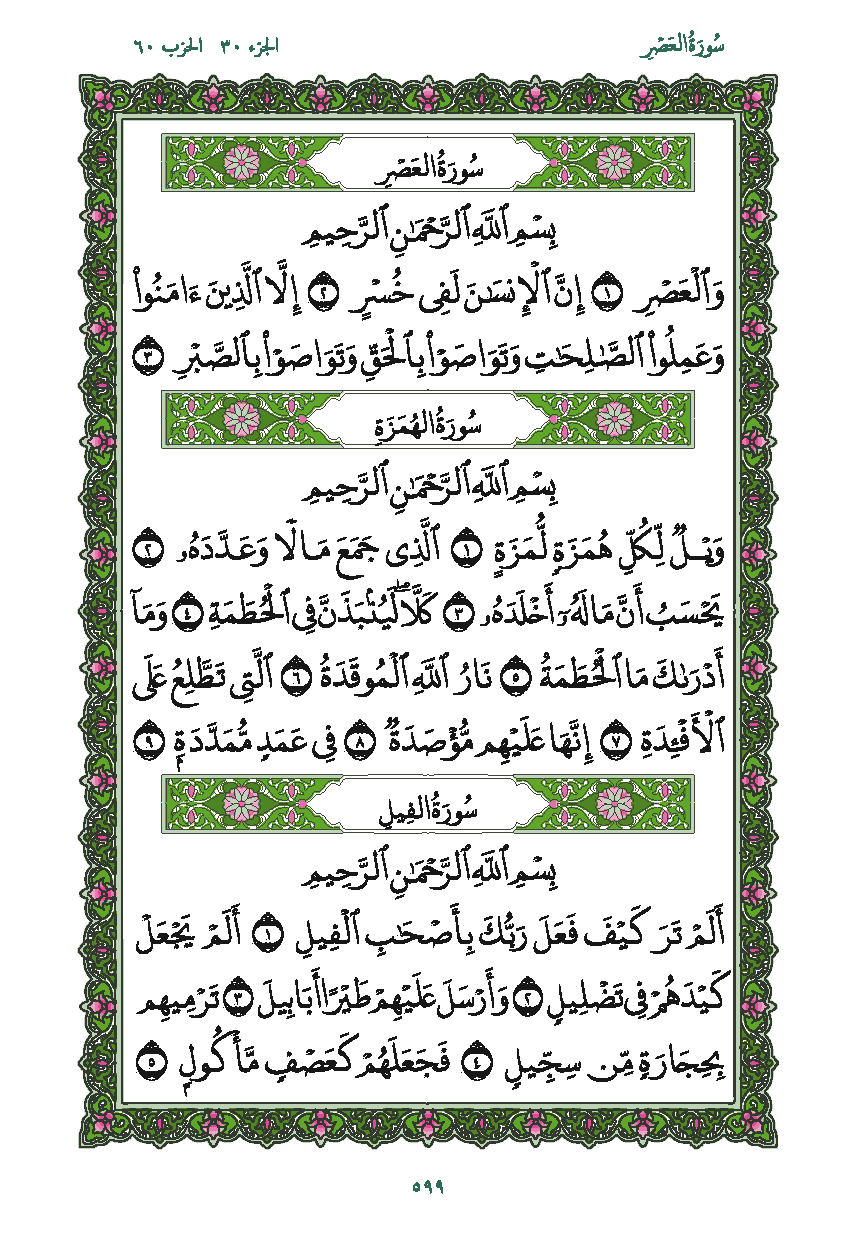
\includegraphics[width=\linewidth,trim=40 40 40 40,clip]{figures/nazm-p599.pdf}
    \caption{Page 599: Al-`Asr, Al-Humaza, Al-Fil.}
  \end{subfigure}\hfill
  \begin{subfigure}[b]{0.3\textwidth}\centering
    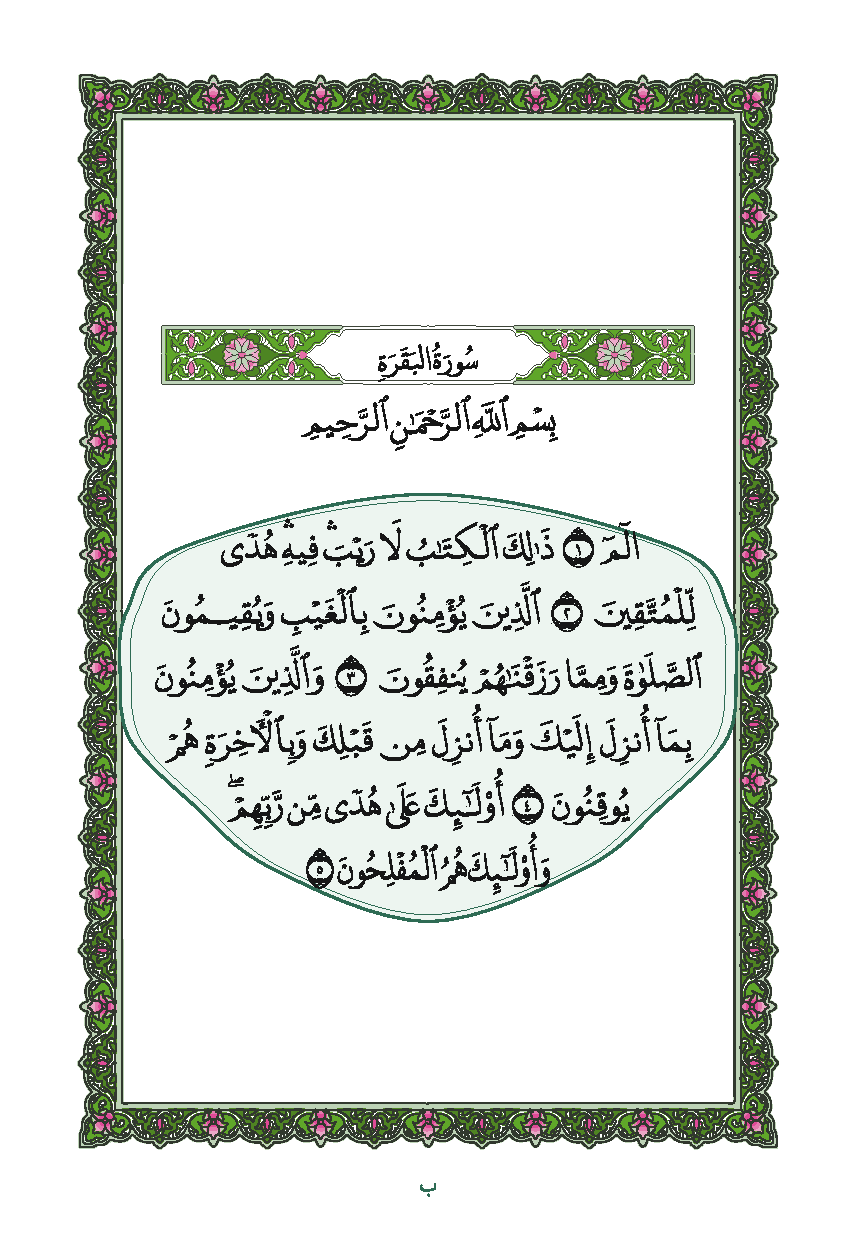
\includegraphics[width=\linewidth,trim=40 40 40 40,clip]{figures/nazm-beh.pdf}
    \caption{Page \emph{b\=a'}: Al-Baqara 1--5.}
  \end{subfigure}\hfill
  \begin{subfigure}[b]{0.3\textwidth}\centering
    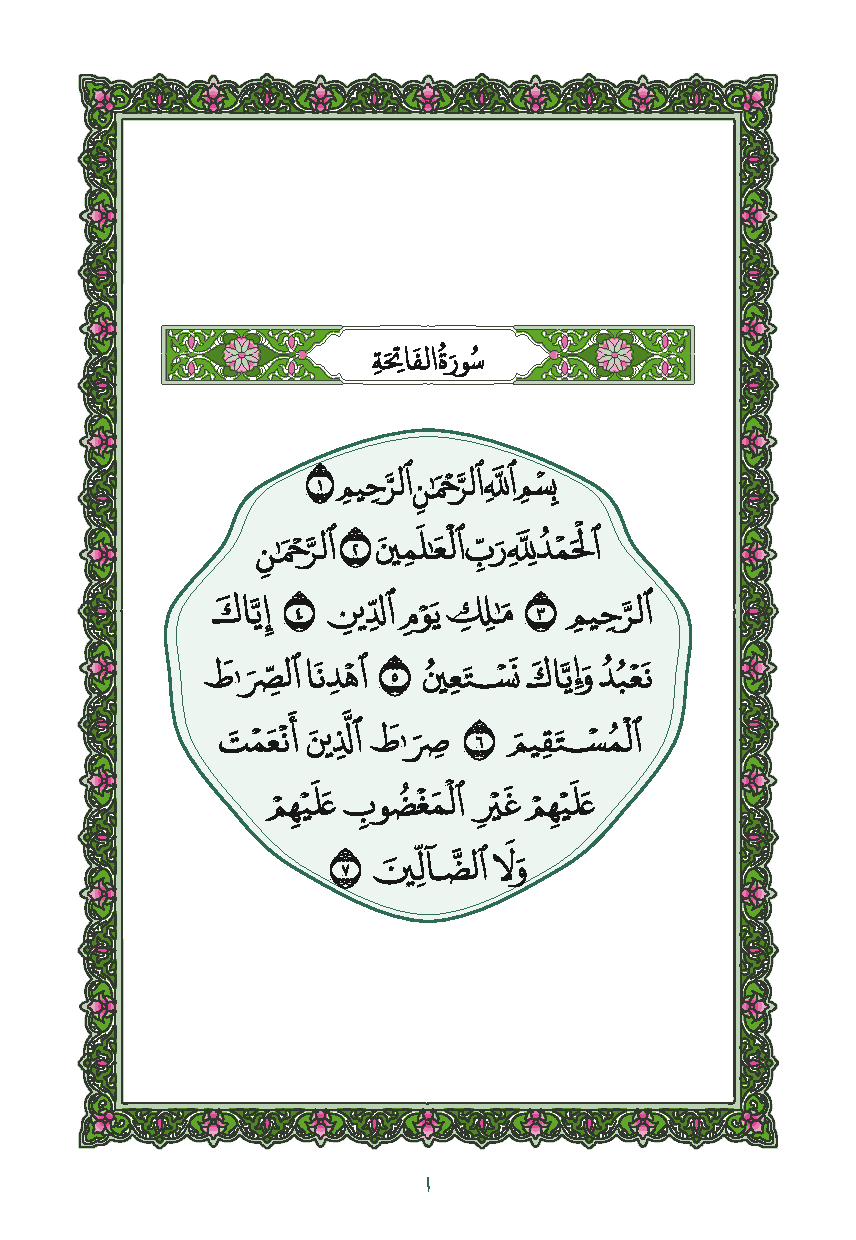
\includegraphics[width=\linewidth,trim=40 40 40 40,clip]{figures/nazm-alef.pdf}
    \caption{Page \emph{alif}: Al-Fatiha.}
  \end{subfigure}
  \Description{Three typeset Quran pages in the green Madina page frame. The left page holds three short surahs, the third title on line 11. The middle and right pages are the opening spread: a surah header above a lens-shaped block of narrowing lines.}
  \caption{Quran-Nazm pages. Right: the opening spread, read right to left, Al-Fatiha and Al-Baqara 1--5 in blocks whose lines narrow towards top and bottom, as in the print. Left: a page of juz 30. Each surah begins on a new line under its header, no title below line~11; every page ends on an ayah.}
  \label{fig:pages}
\end{figure*}
Quran-Nazm~\cite{nazm} is a single Python program, \texttt{render\_mushaf.py}, built on the data and justifier of quran-madina-html~\cite{qmh}. Fig.~\ref{fig:pipeline} shows its stages and Table~\ref{tab:params} its parameters.

\begin{figure}[t]
\centering
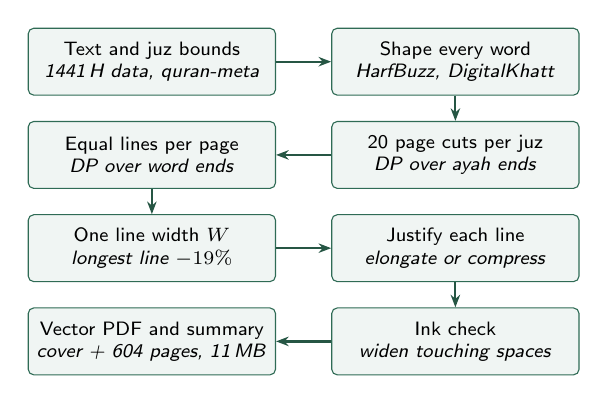
\begin{tikzpicture}[
  box/.style={draw=nazm,rounded corners=2pt,fill=nazm!7,font=\sffamily\scriptsize,align=center,minimum height=8.5mm,text width=30mm,inner sep=2pt},
  arr/.style={-{Stealth[length=1.6mm]},color=nazm!80!black,thick}, node distance=3.2mm and 7mm]
  \node[box] (t) {Text and juz bounds\\\textit{1441\,H data, quran-meta}};
  \node[box,right=of t] (s) {Shape every word\\\textit{HarfBuzz, DigitalKhatt}};
  \node[box,below=of s] (p) {20 page cuts per juz\\\textit{DP over ayah ends}};
  \node[box,left=of p] (l) {Equal lines per page\\\textit{DP over word ends}};
  \node[box,below=of l] (w) {One line width $W$\\\textit{longest line $-19\%$}};
  \node[box,right=of w] (j) {Justify each line\\\textit{elongate or compress}};
  \node[box,below=of j] (c) {Ink check\\\textit{widen touching spaces}};
  \node[box,left=of c] (o) {Vector PDF and summary\\\textit{cover + 604 pages, 11\,MB}};
  \draw[arr] (t)--(s); \draw[arr] (s)--(p); \draw[arr] (p)--(l); \draw[arr] (l)--(w);
  \draw[arr] (w)--(j); \draw[arr] (j)--(c); \draw[arr] (c)--(o);
\end{tikzpicture}
\Description{Flow diagram of eight steps from text and juz boundaries through shaping, page and line cutting, line width, justification and ink check to the vector PDF and its statistics summary.}
\caption{The Quran-Nazm pipeline.}
\label{fig:pipeline}
\end{figure}

\begin{table}[t]
  \centering\small
  \caption{Parameters of the renderer and their defaults.}
  \label{tab:params}
  \begin{tabularx}{\linewidth}{@{}lX@{}}
    \toprule
    Parameter & Meaning (default) \\
    \midrule
    \texttt{-{}-unit} & unit fixed to a page count: \texttt{juz}, 20 pages (juz 30 on 24), or \texttt{hizb}, 10 pages (the last hizb on 14) \\
    \texttt{-{}-shrink} & compression limit $\sigma$ (0.19) \\
    \texttt{-{}-art} & page frame and header art (\texttt{hafs-adi}; \texttt{none} for Nazm's own) \\
    \texttt{-{}-no-cover} & leave out the cover page \\
    \texttt{-{}-pages} & draw only a page range; the layout is always computed for the whole book \\
    \texttt{TITLE\_MAX\_ROW} & lowest line for a surah title (11) \\
    \texttt{JUZ30\_MAX\_STRETCH} & sparsest page allowed in juz 30 (1.35\x) \\
    \texttt{MIN\_SPLIT\_AYAHS} & ayahs kept on each side of a split short surah (2) \\
    \bottomrule
  \end{tabularx}
\end{table}

\paragraph{Text and shaping.} The Hafs text of the 1441\,H layout data~\cite{qmh,tanzil} is split into ayahs and words; rub', hizb and juz boundaries come from quran-meta~\cite{quranmeta}. Every word is shaped once with HarfBuzz in the QMH New Madina font.

\paragraph{Justification.} Lines that are too short are stretched with the DigitalKhatt elongation rules~\cite{anane2021} as ported in quran-madina-html. Lines that are too long tighten their spaces and are then scaled horizontally; the font's shrinking features are never used, nor even tried (Section~\ref{sec:compress}). Lines that would need more than 1.8\x{} stretch (a few words left before a surah ends on a page; 5 in the book) are centred instead.

\paragraph{Juz 30.} Its 37 surahs each start on a new line under a two-line header, so text width is a poor guide to how full a page is. A candidate page is therefore scored by the lines it really needs at width $W$, with cost $(\log \bar s_p)^2$ for its average stretch $\bar s_p$; no page may need more than the compression limit; a split surah keeps at least two ayahs on each page; and splitting a surah that fits on one page costs far more than any imbalance. No page may be sparser than $\bar s_p=1.35$, except the last: under the title rule surahs 112--114 cannot fill it beyond 1.50\x, since a fourth surah would push a title to line 12. The 24 pages are chosen jointly by dynamic programming.

\paragraph{Ink check.} Every set line is tested for ink contact between neighbouring words: glyph boxes that intersect are rasterised at 5 font units per pixel and compared pixel by pixel. Four contacts in the book, of the kind where a small pause mark meets the tall stroke of a following kaf, are cleared by widening only that space and refitting the line.

\paragraph{Output.} A minimal PDF writer stores each glyph outline once as a form object shared by all pages and places it by matrix, which keeps the book, 602 numbered pages and the opening spread, at 11\,MB with vector text. The page frame and surah header are the Hafs al-`Adi vector ornaments of quran-assets~\cite{quranassets}, traced from the Complex's standard Hafs print: each SVG has a transparent slot, the frame's slot is stretched over the text block and the header's holds the surah name, and both are laid under the text as shared form objects. Running heads use Amiri Quran~\cite{amiri}. A static cover, with a short description of the project in Arabic and English, precedes the opening spread. As an Arabic book the file is marked to read right to left (\texttt{/Direction /R2L}) two pages at a time, with the cover alone like a front cover; a two-page viewer then shows the opening spread with Al-Fatiha on the right, and every odd page on the right, as in the print. Page labels name the opening pages \emph{alif} and \emph{b\=a'} and number the rest from~1. Every run also writes a statistics summary, the measures of Section~\ref{sec:results} beside those of the print, so that a reader who changes a parameter sees its effect at once. The whole Mushaf renders in about four minutes on a laptop-class CPU, and a re-run reproduces the published statistics exactly.

\section{Evaluation}\label{sec:results}
All comparisons with the print are measured the same way, on juz 1--29 (juz 30 is an exception in every layout): the stretch of a line is the line width over its natural width, shaped unstretched in DigitalKhatt; for the print, its own full lines; for Nazm, its layout, with centred lines left out. Spreads are standard deviations of $\log s_\ell$; as the line width multiplies every line alike, they do not depend on the type size.

These spreads measure what Nazm optimises. Eqs.~\ref{eq:pages} and~\ref{eq:lines} balance natural widths, so a smaller spread of stretch than the print's, which was never composed to that criterion, is expected rather than discovered; what the spreads show is how much evenness of stretch the rules buy and where in the book (Section~\ref{sec:units-eval}). Section~\ref{sec:texture} adds measures that Nazm does not optimise.

\subsection{Which unit to fix: Madina, 10 pages per hizb, 20 pages per juz}\label{sec:units-eval}
Table~\ref{tab:units3} and Fig.~\ref{fig:variance} compare the print with the two designs of Nazm, each at the same type size (93\% of the print: the hizb design at its 25\% limit, the juz design at 19\%). The spread of all lines splits, in squares, into three parts: between juz, between the pages of a juz, and within a page.

\begin{table*}[t]
  \centering\small
  \caption{The print and the two designs of Quran-Nazm, measured the same way on juz 1--29. Spread: s.d.\ of log stretch; the three indented parts add up in squares to the spread of all lines.}
  \label{tab:units3}
  \begin{tabular}{@{}lccc@{}}
    \toprule
    & Madina 1441\,H & Nazm, 10 pages per hizb & \cellcolor{nazm!10}Nazm, 20 pages per juz \\
    \midrule
    Type size vs the print & 100\% & 93\% & \cellcolor{nazm!10}93\% \\
    Compression limit & by hand & 25\% & \cellcolor{nazm!10}19\% \\
    Median stretch (5th--95th percentile) & 1.00\x{} (0.85--1.19) & 1.07\x{} (0.90--1.28) & \cellcolor{nazm!10}1.07\x{} (0.94--1.22) \\
    Lines more than 10\% compressed & 17\% & 7\% & \cellcolor{nazm!10}2\% \\
    \textbf{Spread of all lines} & 0.104 & 0.108 & \cellcolor{nazm!10}\textbf{0.081} \\
    \quad between juz & 0.047 & 0.049 & \cellcolor{nazm!10}0.049 \\
    \quad between pages of a juz & 0.066 & 0.086 & \cellcolor{nazm!10}\textbf{0.047} \\
    \quad within a page & 0.065 & 0.044 & \cellcolor{nazm!10}0.044 \\
    Spread inside a page (median over pages) & 0.062 & 0.039 & \cellcolor{nazm!10}0.039 \\
    Neighbouring pages (median difference) & 0.051 & 0.044 & \cellcolor{nazm!10}0.039 \\
    Spread between hizbs & 0.050 & 0.085 & \cellcolor{nazm!10}0.051 \\
    Sparsest / densest page & 1.31\x{} / 0.81\x & 1.43\x{} / 0.78\x & \cellcolor{nazm!10}1.32\x{} / 0.88\x \\
    Juz / hizbs starting a page & 26 of 29 / 38 & 30 / 60 & \cellcolor{nazm!10}30 / 34 \\
    Lines squeezed horizontally (whole book) & none & 21\% (max 24\%) & \cellcolor{nazm!10}14\% (max 18\%) \\
    \bottomrule
  \end{tabular}
\end{table*}

\begin{figure}[t]
  \centering
  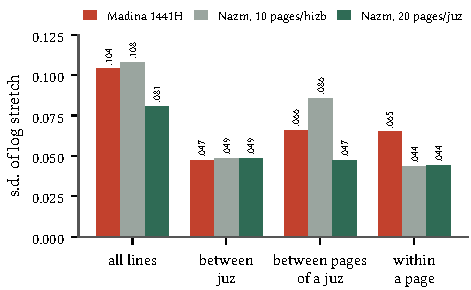
\includegraphics[width=\linewidth]{figures/fig_variance.pdf}
  \Description{Grouped bar chart of the spread of log stretch for the print, the 10-pages-per-hizb design and the 20-pages-per-juz design, in four groups: all lines (0.104, 0.108, 0.081), between juz (0.047, 0.049, 0.049), between pages of a juz (0.066, 0.086, 0.047) and within a page (0.065, 0.044, 0.044).}
  \caption{Where each layout leaves the root variance. Fixing the hizb evens lines within a page but makes the pages of a juz less even than the print; fixing the juz evens both.}
  \label{fig:variance}
\end{figure}

Both designs even out lines within a page by about a third, because both choose a page's line breaks together. They differ between pages. Fixing every hizb to ten pages makes each hizb absorb its own length: a short hizb is stretched over all its ten pages, a long one compressed, and the page-to-page spread inside a juz rises to 0.086, \emph{above} the print's 0.066. Over all lines the hizb design is then no more even than the print (0.108 against 0.104), although every one of its pages looks better than the print's from inside. Fixing only the juz removes this: hizbs start wherever the text puts them, the pages of a juz carry equal shares, and the page-to-page spread falls to 0.047, 28\% below the print. The spread of all lines falls 22\% below the print. The spread between juz is the same in all three layouts (0.047--0.049), since all three fix the juz; it is the root variance that remains.

The price of the juz design is the hizb alignment: 34 of the 60 hizbs start at the top of a page, against all 60 in the hizb design and 38 in the print. Since the juz design also reaches the same type size at a lower compression limit, it squeezes fewer lines (14\% against 21\%) and less (at most 18\% against 24\%).

\subsection{Comparison with the print}
Table~\ref{tab:results} summarises the render against the print, and Fig.~\ref{fig:stretch} shows the distributions. The key measure of harmony within a page, the median over pages of the spread of $\log s_\ell$, falls from 0.062 to 0.039 ($-37\%$). Every page ends on an ayah, no line opens with a marker, no surah title sits below line 11, and no two words touch.

\begin{table}[t]
  \centering\small
  \caption{Madina 1441\,H print and Quran-Nazm (juz 1--29 for the spreads; whole book otherwise).}
  \label{tab:results}
  \begin{tabularx}{\linewidth}{@{}Xcc@{}}
    \toprule
    & Madina & Nazm \\
    \midrule
    Pages & 604 & 604 (+ cover) \\
    Fixed unit & juz $\to$ 20 pages & juz $\to$ 20 pages \\
    Type size & 100\% & 93\% \\
    Spread of all lines & 0.104 & \textbf{0.081} \\
    Spread between pages of a juz & 0.066 & \textbf{0.047} \\
    Spread inside a page & 0.062 & \textbf{0.039} \\
    Median line stretch & 1.00\x & 1.07\x \\
    Lines more than 10\% compressed & 17\% & 2\% \\
    Lines opening with a marker & 6.5\% & 0 \\
    Surah titles below line 11 & 5 & 0 \\
    Pen weight across lines & $\pm$13\% & even on 86\% of lines \\
    Lines squeezed horizontally & none (pen) & 14\% (max 18\%) \\
    \bottomrule
  \end{tabularx}
\end{table}

\begin{figure}[t]
  \centering
  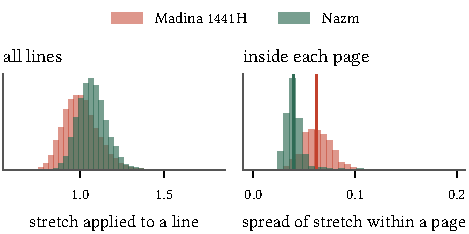
\includegraphics[width=\linewidth]{figures/fig_stretch.pdf}
  \Description{Two overlaid histograms comparing the print and Nazm: line stretch overall, where Nazm is shifted slightly higher and narrower, and the spread of stretch within each page, where Nazm is clearly narrower.}
  \caption{Stretch applied to each line (left) and its spread within each page (right), print vs Nazm, juz 1--29. Vertical lines mark the medians (0.062 and 0.039). Nazm's lines are more alike overall; their slight shift towards stretching is the cost of type at 93\% of the print, chosen to keep horizontal squeezing rare.}
  \label{fig:stretch}
\end{figure}

The price is visible in two places. Nazm stretches more on average (median 1.07\x): type at 93\% leaves the median line a little short of the width, a choice made to limit squeezing, since at the print's own size (25\% limit) nearly half the lines would be squeezed (Table~\ref{tab:shrink}). And one line in seven is compressed partly by horizontal scaling. Both trace to the compression side of the font, which elongates gracefully but has no safe way to contract a word inside a line.

\subsection{Measures Nazm does not optimise}\label{sec:texture}
Table~\ref{tab:texture} compares texture measures that play no part in Nazm's objective, on the same lines. The print is measured on the DigitalKhatt reproduction fitted to its lines in quran-madina-html (each word's elongation alternates, each line's word gaps, narrowed words and scale), so these are properties of the reproduction, not of the pen strokes. Elongation is the width each word gains from its elongation features, shaped with and without them in the same font.

\begin{table}[t]
  \centering\small
  \caption{Texture measures not optimised by Nazm (juz 1--29). Shares are of the line width; print: its DigitalKhatt reproduction.}
  \label{tab:texture}
  \begin{tabularx}{\linewidth}{@{}Xcc@{}}
    \toprule
    & Print & Nazm \\
    \midrule
    Words per line, mean (s.d.) & 8.8 (1.5) & 8.8 (1.4) \\
    Elongated words per line & 2.5 & 1.3 \\
    Lines with any elongation & 65\% & 45\% \\
    Elongation share, mean (95th pct.) & 7.3\% (23\%) & 3.1\% (13\%) \\
    Word gap share, median (5th--95th pct.) & 0.94\% ($-$0.43--1.37\%) & 1.21\% (0.36--1.40\%) \\
    Lines with narrowed words & 15\% & 0 \\
    Lines scaled horizontally & 0.2\% & 14\% \\
    \midrule
    \multicolumn{3}{@{}l}{\emph{Distortion: letters scaled horizontally by $k<1$}} \\
    Lines distorted (by more than 5\%) & 15\% (7.1\%) & 14\% (4.3\%) \\
    $1-k$ on those lines, mean (95th pct.) & 5.8\% (15\%) & 4.0\% (11\%) \\
    $1-k$, worst line & 27\% & 18\% \\
    $1-k$, mean over all lines & 0.9\% & 0.6\% \\
    \bottomrule
  \end{tabularx}
\end{table}

The measures cut both ways. Nazm elongates less than half as much as the reproduction of the print, on fewer lines, and its word gaps vary less from line to line. But its gaps are wider (a median of 1.21\% of the line against 0.94\%), a looser texture that follows from type at 93\% and from widening spaces before letters; and where the reproduction fits 15\% of the print's lines by narrowing individual words, Nazm fits 14\% of its lines by scaling the whole line (Section~\ref{sec:compress}).

The evenness metric of this section is blind to this: a squeezed line counts at its target width, whatever it costs the letters. So the table also reports distortion beside it. A horizontal scale $k$ narrows every letter of the line and thins its vertical strokes by $1-k$, while horizontal strokes keep their weight, so a scaled line is both narrower and lighter in its uprights than its neighbours. Nazm distorts 14\% of its lines, by 4.0\% on average and 18\% at worst; 4.3\% of lines are scaled by more than 5\%. These are not small: at 18\% the thinning is of the order of the $\pm$13\% pen-weight differences we measured on the print (Section~\ref{sec:pen}), and it falls on single lines rather than drifting across a page. For the print the same figures describe its DigitalKhatt reproduction, which must narrow words on 15\% of lines (up to 27\%) to match what the calligrapher wrote; they say how far the print departs from the font's natural forms, not that its pen strokes are distorted. We therefore claim no advantage in distortion, only that Nazm's is bounded by the 19\% limit and confined to one line in seven.

\subsection{Ablations and the exact optimum}\label{sec:ablation}
Table~\ref{tab:ablation} isolates the optimisers on juz 1--29. Each variant computes its own line width at $\sigma=19\%$.

\begin{table}[t]
  \centering\small
  \caption{Ablations (juz 1--29, $\sigma=19\%$). In page: median over pages of the spread of log stretch; between: spread between pages of a juz; sparsest: highest average stretch of any page.}
  \label{tab:ablation}
  \begin{tabularx}{\linewidth}{@{}Xccccc@{}}
    \toprule
    Variant & Type & In page & Between & Sparsest & Squeezed \\
    \midrule
    \rowcolor{nazm!10} Nazm (joint pages, joint lines) & 93\% & 0.039 & 0.047 & 1.32\x & 14\% \\
    Greedy page cuts & 83\% & 0.039 & 0.070 & 1.88\x & 2\% \\
    Greedy page and line cuts & 83\% & 0.057 & 0.070 & 1.88\x & 2\% \\
    \bottomrule
  \end{tabularx}
\end{table}

\paragraph{Joint page cuts keep pages even.} Cutting each page at the ayah end nearest to its share lets the error of each cut carry into the next; over nineteen cuts per juz some pages end up far too full or too empty. The spread between pages rises from 0.047 to 0.070, the sparsest page reaches 1.88\x, and the overfull pages set the line width, so type falls from 93\% to 83\%. With twenty pages per juz, joint page cuts (Eq.~\ref{eq:pages}) matter more than they did with ten per hizb, where greedy cuts cost only three points of type size.

\paragraph{Joint line cuts reduce the spread within a page.} Cutting each line at the word nearest to its share leaves lines up to half a word off target; with about nine words per line that is $\pm$5--10\%. Choosing all of a page's line breaks together (Eq.~\ref{eq:lines}) lowers the spread from 0.057 to 0.039.

\paragraph{How far from the optimum?} The two-stage method balances pages by text width and then breaks lines; it does not see the integer effects of whole lines per surah segment and of word granularity when it places page breaks. We solved the joint problem exactly: minimise $\sum_\ell(\log s_\ell)^2$ over all lines of a juz, with page and line breaks chosen together under all the rules. The problem is a chain, so nested dynamic programming finds the true optimum: for each candidate page, the best cut of each surah segment into $n$ lines and the best share of the page's lines among its segments, then the best twenty pages as a shortest path with exactly twenty arcs. We checked its page level against the same problem stated as an integer programme and solved with HiGHS~\cite{huangfu2018}; the optima agree to every digit. At the final line width the exact optimum improves the two-stage objective by only 2.8\% (92.4 against 95.0), and on the hizb design by 2.4\%. The two-stage method is thus close to optimal, and far cheaper.

\subsection{Between juz}
Fixing every juz to twenty pages moves the root variance of Section~\ref{sec:units} into the average stretch of each juz (Fig.~\ref{fig:juzstretch}). Juz~10, whose text is short for twenty pages, averages 1.16\x; juz~29, the densest once its many surah headers are counted, averages 0.93\x. The spread between juz is 0.049, the same as in the print (0.047). This difference is gradual: a reader meets it only by comparing distant parts of the book, never within a spread.

\begin{figure}[t]
  \centering
  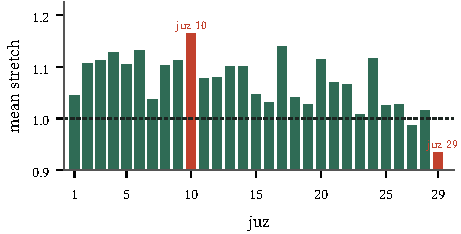
\includegraphics[width=\linewidth]{figures/fig_juz_stretch.pdf}
  \Description{Bar chart of the mean stretch of each of juz 1 to 29, mostly between 1.0 and 1.15, with juz 10 the highest at about 1.16 and juz 29 the lowest at about 0.93.}
  \caption{Mean line stretch of each juz in Nazm: the root variance, absorbed juz by juz.}
  \label{fig:juzstretch}
\end{figure}

\subsection{Surah titles, extremes and juz 30}\label{sec:extremes}
\paragraph{The title rule.} Without it, 11 surah titles of juz 1--29 would sit on line 12 or 13. The rule moves page breaks on 107 pages, since a moved break shifts the rest of its juz, but changes no spread (0.039 within a page, 0.047 between pages) and lowers the sparsest page from 1.38\x{} to 1.32\x: without the rule the sparsest page of the book (page~479) is one where a surah opens at its foot.

\paragraph{Extremes.} Fig.~\ref{fig:extremes} shows the two extreme pages of juz 1--29. Page~119 (Al-Ma'ida 82--89) is the densest, at 0.88\x{} average stretch; its lines are narrowed by tighter spaces and some horizontal scaling. Page~43 (Al-Baqara 270--274) is the sparsest, at 1.32\x; its lines carry long elongations but no distortion. Both are milder than the extremes of the hizb design (0.78\x{} and 1.43\x) and of the print (0.81\x{} and 1.31\x{} measured the same way).

\begin{figure}[t]
  \centering
  \begin{subfigure}[b]{0.48\linewidth}\centering
    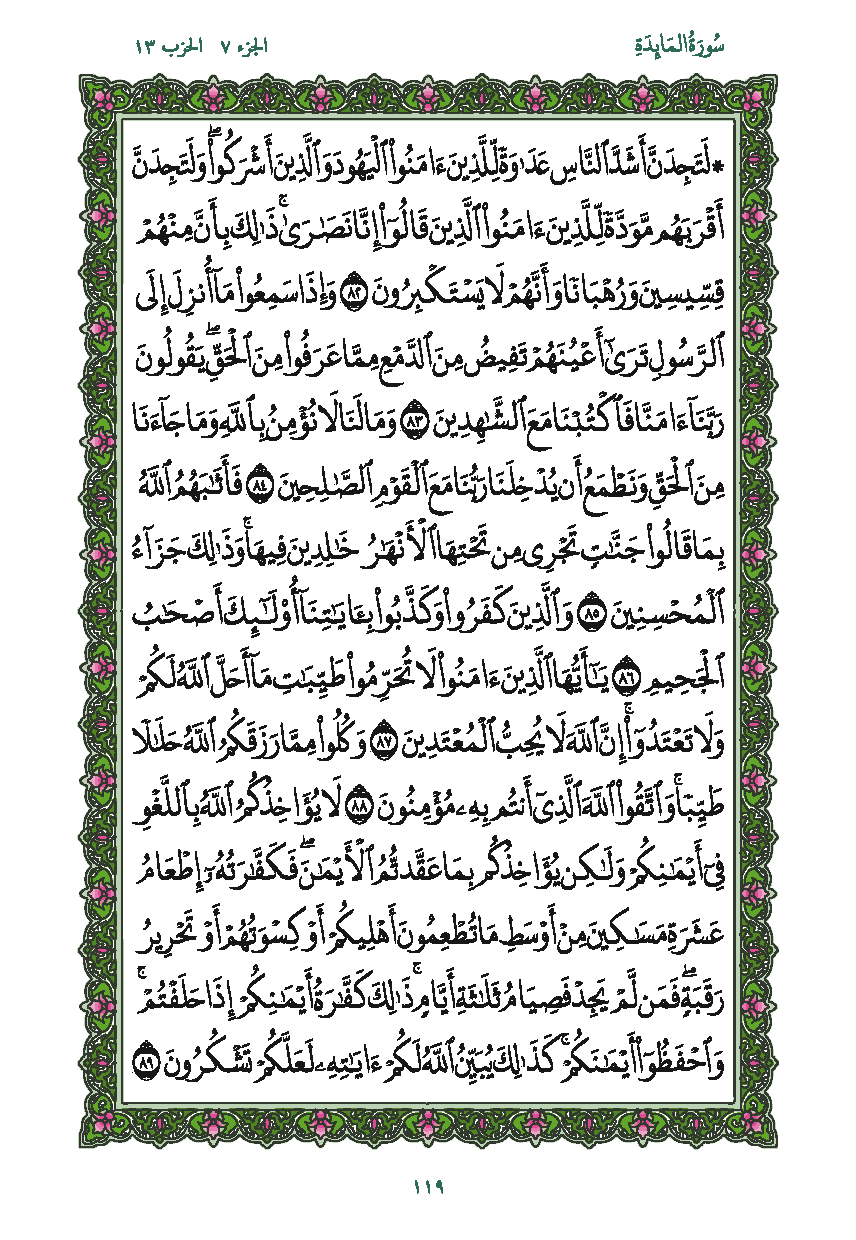
\includegraphics[width=\linewidth,trim=40 40 40 40,clip]{figures/nazm-p119.pdf}
    \caption{Page 119, densest.}
  \end{subfigure}\hfill
  \begin{subfigure}[b]{0.48\linewidth}\centering
    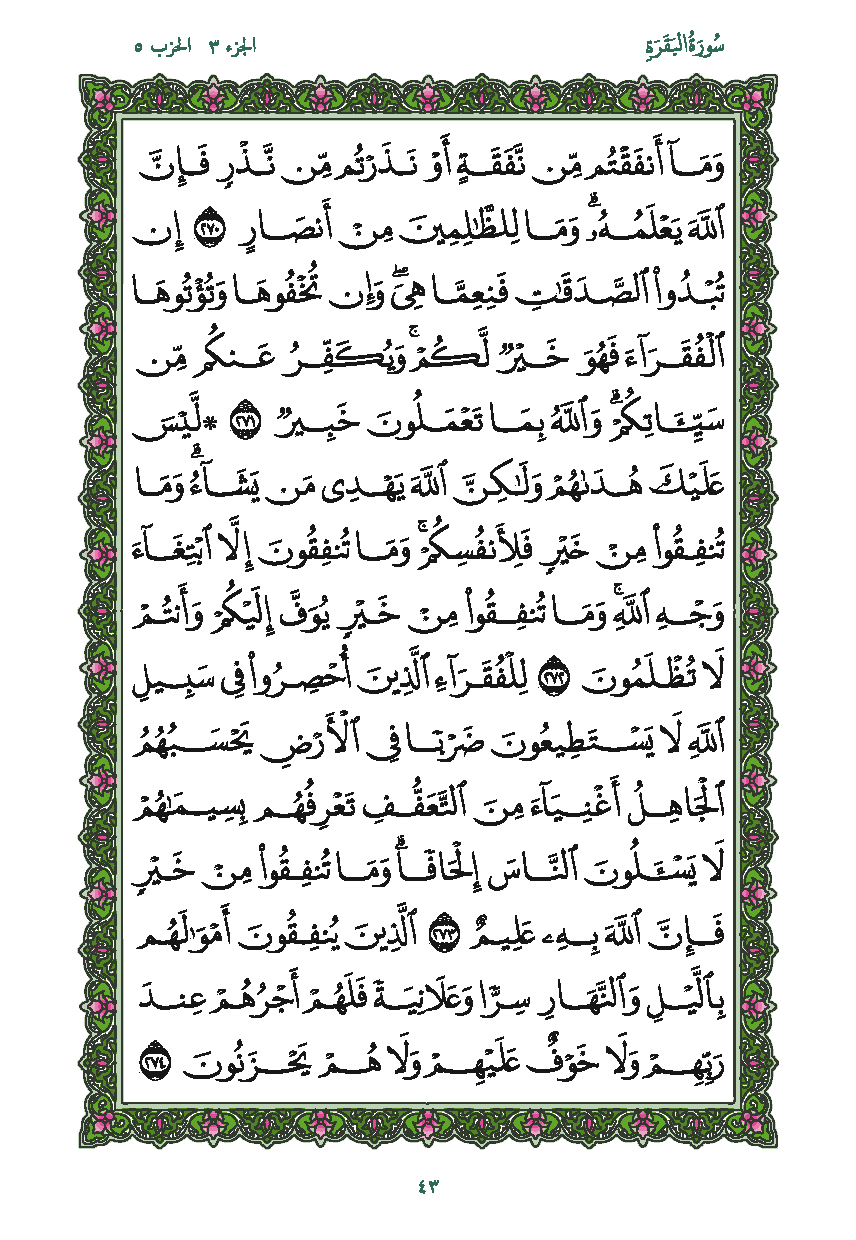
\includegraphics[width=\linewidth,trim=40 40 40 40,clip]{figures/nazm-p043.pdf}
    \caption{Page 43, sparsest.}
  \end{subfigure}
  \Description{Two Nazm pages side by side: on the left a dense page whose lines are slightly compressed, on the right a sparse page with long letter elongations.}
  \caption{The two extreme pages of juz 1--29 in Nazm.}
  \label{fig:extremes}
\end{figure}

\paragraph{Juz 30.} Table~\ref{tab:juz30} shows how its rules interact. Twenty pages cannot hold its 37 surahs within the rules; 24 pages can, with every page between 0.88\x{} and 1.55\x{} and four short surahs (86, 92, 98, 100) split across two pages, each with at least two ayahs per page. Surahs 103--114 are twelve surahs of one to four lines: with every title at line 11 or higher a page holds at most three of them, so they take exactly four pages, the sparsest of the juz; the last page (112--114) is the same as in the print. Letting a surah that starts and ends on the same page open lower relieves the tightest of these pages and leaves one title on line 12; a 25th page changes nothing. Without the title rule, the last page is no longer exempt from the 1.35\x{} sparsity cap, and no 24-page layout keeps every page within it at the 19\% limit.

\begin{table}[t]
  \centering\small
  \caption{Juz 30 variants at $\sigma=19\%$. Range: lowest and highest average stretch of a page; splits: surahs that fit on one page but span two; low titles: below line 11.}
  \label{tab:juz30}
  \begin{tabularx}{\linewidth}{@{}Xccc@{}}
    \toprule
    Variant & Range & Splits & Low titles \\
    \midrule
    20 pages, title rule & \multicolumn{3}{c}{no layout} \\
    24 pages, no title rule & \multicolumn{3}{c}{no layout (sparsity cap)} \\
    \rowcolor{nazm!10} 24 pages, title rule & 0.88--1.55\x & 4 & 0 \\
    24 pages, whole surah may open lower & 0.88--1.52\x & 4 & 1 \\
    25 pages, title rule & 0.88--1.55\x & 4 & 0 \\
    \bottomrule
  \end{tabularx}
\end{table}

\section{Reproducibility}\label{sec:repro}
Everything in this paper is generated from public inputs by the scripts in the Quran-Nazm repository~\cite{nazm}: the text and layout data and the DigitalKhatt fonts of quran-madina-html~\cite{qmh}, the reading-unit boundaries of quran-meta~\cite{quranmeta}, the King Fahd Complex PDF~\cite{scan} for the scan measurements, and the QCF4 word glyphs~\cite{qcf4} for the check of the yardstick and the vector pen-weight measurements. Numbered scripts reproduce each measurement (line density, pen weight, ayah markers, unit lengths, the design studies, the ablations, the title rule, the exact optimum and the three-way comparison) and write their results to JSON files in the repository; \texttt{render\_mushaf.py} produces the Mushaf, its statistics summary, a full report and the page layout; and a separate script rebuilds every figure of the paper. The renderer is deterministic: re-running it reproduces the published report exactly. Its parameters (Table~\ref{tab:params}) make the alternatives of this paper one command each, the hizb design included.

\section{Limitations and future work}\label{sec:limits}
\paragraph{Compression.} One line in seven is compressed partly by horizontal scaling. The font offers no safe narrow forms today (Section~\ref{sec:compress}); a set of compression forms in DigitalKhatt that keep letters clear inside a full line (narrower alternates, tighter ligatures, shorter tails), or a reviewed subset of the existing \texttt{shrr} tucks, would remove most of it and allow type at the print's size.

\paragraph{Hizb alignment.} Fixing only the juz gives up the alignment of hizbs with page tops (34 of 60). A middle way, hizbs of nine to eleven pages as in the print within a fixed juz, would keep more hizbs at a page top at a small cost in page evenness; it is a design question for readers and teachers who navigate by hizb.

\paragraph{Expert review.} Our measures are geometric. A judgement of evenness, legibility and beauty is still needed, but a blind study with ordinary readers is not realistic: most readers know the pages of the Madina Mushaf by heart and would recognise its pages, and Nazm's, at a glance. We therefore plan to put paired pages before experienced evaluators, the scholars of the committees that review and approve printed Mushaf editions, who see many layouts of the same text and judge them against the conventions of the tradition rather than against a remembered page.

\paragraph{Other narrations.} Quran-Nazm sets the Hafs narration from `Asim. Nothing in the method is specific to it: given a narration's text with its ayah and reading-unit boundaries, and a font for its script conventions, the same rules apply. A natural extension is to the other narrations, starting with those already printed by the King Fahd Complex (such as Warsh and Qalun from Nafi`, and al-Duri from Abu `Amr), and then to all twenty narrations of the ten canonical readings, so that each can have an evenly set Mushaf from one open program. Each brings its own text, its own ayah count and unit boundaries, and, for some, a different hand to model in the font.

\paragraph{Design.} The page frame and surah headers reuse the ornaments of the Complex's standard Hafs print, traced as vector art by quran-assets; their licence is provisional until the Complex grants permission, so the renderer keeps its own frame and headers as an alternative. The title rule still lets a surah open on line 11 with three lines before a page turn; a stricter limit for surahs that continue on the next page would remove those. The treatment of juz~30 is open to calligraphers' review. Redefining the reading units to equal lengths would remove the root variance, but that is beyond the typesetter's remit.

\section{Conclusion}
Unequal reading units are the root of layout variance in every Mushaf. The Madina print fixes the juz, the most forgiving unit, and absorbs the rest by hand: a third of its lines are off their natural length by over 10\%, and stroke weight follows the crowding. A stricter unit is tempting, since every hizb would then begin on a known page, but fixing every hizb to ten pages leaves the pages of a juz less even than the print. Quran-Nazm keeps the print's unit and absorbs the variance by explicit rules on shaped text widths: every page ends on an ayah, no surah title falls below line 11, no word collides with its neighbour, and the spread of line stretch falls by 22\% over the book, 28\% between pages and 37\% within a page. The program, data, measurements and the rendered Mushaf are available under a dual Waqf\,2.0/commercial licence~\cite{nazm}; the frame and header art keeps its own CC BY-NC-SA~4.0 terms.

\begin{acks}
This work builds on DigitalKhatt by Amine Anane, the Tanzil project, HarfBuzz, fontTools~\cite{fonttools}, quran-meta, HiGHS and Amiri. The page frame and surah header art comes from quran-assets by quran.ws (CC BY-NC-SA~4.0). The Madina Mushaf images are reproduced from the King Fahd Complex edition for analysis.
\end{acks}

\bibliographystyle{ACM-Reference-Format}
\bibliography{refs}

\end{document}
